
%  $Description: Author guidelines and sample document in LaTeX 2.09$  $Author:
% ienne $ $Date: 1995/09/15 15:20:59 $ $Revision: 1.4 $

\documentclass[times, 11pt,twocolumn]{article}
\usepackage{latex8}
\usepackage{times}
\usepackage{graphicx}
\usepackage{listings}
\usepackage{epsfig}



% ------------------------------------------------------------------------- take
% the % away on next line to produce the final camera-ready version
\pagestyle{empty}

% -------------------------------------------------------------------------
\begin{document}
\lstset{language=Haskell, numbers=left,
numberstyle=\tiny,numbersep=5pt,basicstyle=\scriptsize,aboveskip=20pt}

\title{Towards a Crosscutting Approach for Variability Management}

\author{Rodrigo Bonif\'{a}cio and Paulo Borba\\
Informatics Center \\ Federal University of Pernambuco \\ Recife, Brazil \\
\{rba2, phmb\}@cin.ufpe.br\\ }

\maketitle
\thispagestyle{empty}

\begin{abstract}
   The ABSTRACT is to be in fully-justified italicized text, at the top 
   of the left-hand column, below the author and affiliation 
   information. Use the word ``Abstract'' as the title, in 12-point 
   Times, boldface type, centered relative to the column, initially 
   capitalized. The abstract is to be in 10-point, single-spaced type. 
   The abstract may be up to 3 inches (7.62 cm) long. Leave two blank 
   lines after the Abstract, then begin the main text. 
\end{abstract}



%------------------------------------------------------------------------- 
\Section{Introduction}\label{sec:intro}

In order to reduce time-to-marketing and improve quality of software products,
several approaches and techniques for economy of scope, mass customization, and
systematic reuse have been recently proposed. Examples of such approaches include \emph{Software Product
Lines}~\cite{Pohl:2005aa, Clements:2001aa}, \emph{Generative Programming
Techniques}~\cite{Czarnecki:2000aa}, and \emph{Software
Factories}~\cite{Greenfield:2003aa}. Actually, there is a lot in common among
such approaches. For instance, one common characteristic is the relevance of
domain analysis, which aims at defining a scope (often in the business sense)
in which reusable assets can be used for generating specific products.

Additionally, it is a common practice to use \emph{feature modeling} for
representing features that are common to all products within a scope and which
features are optional, being useful for diferentiating specific products in a
family. Therefore, aiming to generate specific products, it would be necessary
to: (a) introduce suitable variation points in common assets, (b) develop
variant assets that extend these variation points, and (c) relate features to both common and
variant assets.

In this work, we consider \emph{variability management} as the discipline that
guides these activities. Actually, variability management is an interesting kind
of crosscutting concern, since certain features require variation points to be
spread in different places of requirements, design, code, and test artifacts.
This crosscutting nature of variability management results in interesting
challenges regarded to SPL traceability, evolvability, and product derivation. As
a consequence, several authors have proposed the use of \emph{aspect-oriented}
techniques to better modularize the composition of common and variant assets of a
product line~\cite{}. In this thesis we go beyond this composition issue. We
mainly consider a more encompassing notion of variability management, presenting
its semantics as a crosscutting concern and describing the contribution of
relevant artifacts (such as feature models and configuration knowledge) in
product generation.

Our hypotheses is that a clear separation between variability management and
common software engineering artifacts improves SPL evolvability, traceability,
and product derivation. A clear separation means that each SPL model (feature
model, configuration knowledge, SPL use case model, and so on) should focus on
specific concerns. For instance, use case models should represent just the valid
interactions with a software. They should not be enriched to describe variability
space (as proposed in~\cite{Bertolino:2003aa}). The challenge is that, in order
to generate specific products, the clear separation that we are proposing
requires composition processes involving different SPL models. In this thesis,
we define the semantics of composition processes as crosscutting mechanisms.
The elegant notion of crosscutting mechanisms, formalized by Masuhara and
Kiczales~\cite{Masuhara:2003aa}, is used as underlining support for presenting
the semantics of our composition processes. 

Initial results of our approach, applied in the context of representing SPL
variabilities in use case scenarios, revealed to us improvements in both
evolvability and product generation~\cite{Bonifacio:2008aa}. The choice of applying our
approach in this context was motivated because current techniques for scenario variability
management~\cite{Eriksson:2005aa, Bertolino:2003aa} do not present a clear
separation between variability management and scenario specification.
In summary, the contributions of this thesis are threefold

\begin{itemize}
 \item Characterize the broader notation of variability management as
a crosscutting concern and, in this way, propose an approach for
representing it as an independent view of the SPL. Although
this work focuses on requirements artifacts, more specifically
use case scenarios, we argue that such separation is also required
in other SPL models.
 \item A framework for modeling the composition processes of scenario
variability mechanisms. This framework gives a basis for
describing variability mechanisms (such as scenario composition
and parameterization), allowing a better understanding of each mechanism and
highlighting the contribution of each model used in the composition processes.
In this work, such a framework is used for modeling the semantics of scenario variability mechanisms, but it
might be customized for other SPL views.
 \item A deeper evaluation of existing techniques for representing scenario
 variability. Such an evaluation will take into consideration not only the
 support for different variability techniques (parameterization, optional
 scenarios), but also a comparison of existing works with regard to
 SPL evolvability and traceability.  
\end{itemize}

The next section describes our approach, named as \emph{variability management
as crosscutting} (Section~\ref{sec:vmcc}). It also relates some open questions
of our aproach, which we are going to solve in this thesis. After that,
Section~\ref{sec:evaluation} presents the results of three empirical studies,
which we have compared our proposed approach with existing
works. These comparisons were based on \emph{Design Structure Matrices} and on a
suite of metrics, addapted from aspect-oriented communit, for quantifying modularity.
We also present in Section~\ref{sec:evaluation} a discussion about several
improvements on our evaluation processes. Then, we relate our
thesis with existing works (Section~\ref{sec:related}) and present final concludings 
in Section~\ref{sec:concludings}.

%-------------------------------------------------------------------------
\section{Variability management as crosscutting}\label{sec:vmcc}

As we said in the previous section, we are proposing an approach for
variability management that aims to separate variability models
from common software engineering models. However, once these concerns 
had been saparated, it would be necessary to weave those models in order to 
generate specific products. Moreover, in this work we consider variability
management as a crosscutting concern, since certain features require variation
points to be spread in different places of SPL artifacts. 

In order to represent variability management as a crosscutting concern, we
proposed a modeling framework (Section~\ref{sub:framework}), that slightly
generalizes the Masuhara and Kiczales (MK) framework~\cite{Masuhara:2003aa}, and instantiate it for the 
product line domain. The MK framework aims to explain
how different \emph{aspect-oriented} technologies support crosscutting
modularity. In their proposed approach, each technology is modeled as a
three-part description: the related weaving processes take two programs as input, 
which crosscut each other with respect to the resulting program or
computation~\cite{Masuhara:2003aa}.

Specifically in the context of use case scenario variabilities, we represent the
semantics of \textbf{scenario variability management} as a weaver that takes as input four specifications
(\emph{product line use case model}, \emph{feature model}, \emph{product
configuration}, and \emph{configuration knowledge}) that crosscut each other with
respect to the resulting product specific use case model
(Figure~\ref{fig:weave-process}). Combining these input languages, it is possible
to represent the kinds of variability that we are interested in: \emph{optional
use cases and scenarios}, \emph{quantified changed scenarios}, and
\emph{parameterized} scenarios.

\begin{figure}[t]
 \begin{center}
  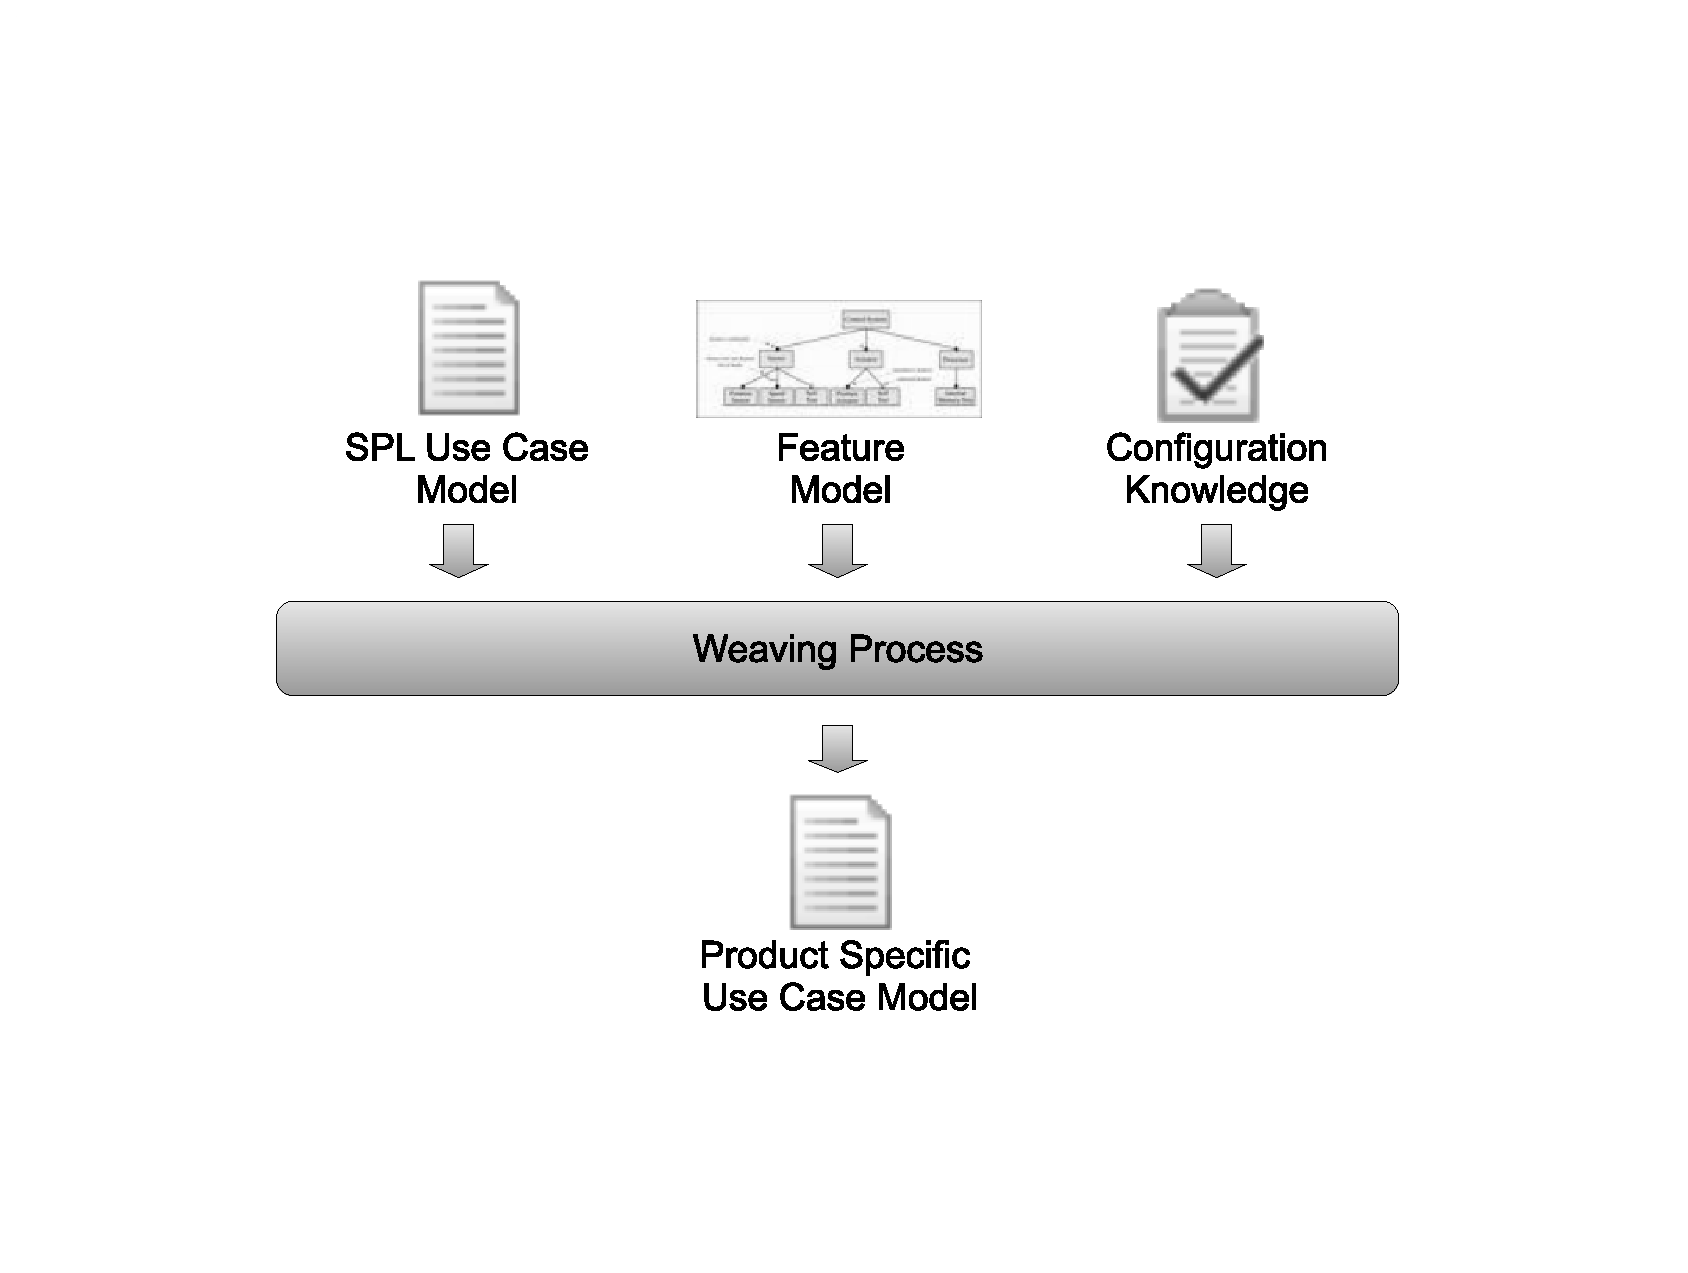
\includegraphics[scale=0.35]{../images/weave-process.eps}
  \caption{Overview of our weaving process.}
  \label{fig:weave-process}
  \end{center}
\end{figure}

In what follows, we present our modeling framework, proposed to explain
variability management as a crosscutting concern. Then, we instantiate such a
framework (Section~\ref{sub:framework-instance}) for representing one scenario
variability technique --- optional use cases and scenarios. More details about our approach can be found
elsewhere~\cite{}.

\subsection{Modeling framework}\label{sub:framework}

As explained before, our modeling framework, proposed for representing 
variability management weaving processes, is based on the Masuhara and Kiczales
work~\cite{Masuhara:2003aa}. Thereby, we describe each variability technique
as a weaver. In our work, we represent these weavers as an
\emph{6-tuple} (see Eq.~\ref{eq:tuple} and Table~\ref{tab:tup-01}), in
such a way that we can describe the contribution of each input model used 
in the composition process (Figure~\ref{fig:weave-process}).

\begin{equation}
Weaver = \{o, o_{jp}, L, L_{id}, L_{eff}, L_{mod}\}, 
\label{eq:tuple}
\end{equation}

\begin{table}[bth]
\begin{center}
\caption{Modeling framework elements.} \label{tab:tup-01}
\begin{tabular}{|p{0.6in}|p{2.4in}|}
  \hline
  {\bf Element} & {\bf Description} \\ 
   \hline
  $o$          & Output language used for describing the results of the weaving process \\ \hline
  $o_{jp}$     & Set of join points in the output language \\ \hline
  $L$          & Set of languages used for describing the input specifications \\ \hline
  $L_{ID}(l)$  & Set of constructions in each input language $l$, used for identifying the output join points \\ \hline 
  $L_{EFF}(l)$ & For each input language $l$, this element represent the effect of its constructions in the weaving process \\ \hline
  $L_{MOD}(l)$ & Set of modular unities of each input language $l$\\ \hline
  \hline
\end{tabular}
\end{center}
\end{table}

As a consequence, we model each variation technique by filling in
the six parameters of our \emph{6-tuple} representation. In order to do
that, we first provide a reference implementation for the corresponding
weaver. After that, we state how elements of the reference implementation
correspond to elements of the modeling framework. In this way, we can represent the semantics
of a variability technique at the same time that we explain the contribution of each involved model. 
Altogether, by applying our approach, it is possible to design variation
techniques that present a better separation between variability models and
common software engineering artifacts.

In our case studies, we are representing the reference implementations (and the
meta-model of the input and output models) using the Haskell programming language. 
This leads to concise weaving processes descriptions and keeps our model close
to MK work, where weaving processes are specified in the Scheme programming language. 

%-------------------------------------------------------------------------------
\subsection{Modeling framework instance}\label{sub:framework-instance}

In this section we present an instance of our modeling framework. This
instance describes the variation technique responsible for selecting, based on a specific product
configuration, which scenarios will be assembled in a product.
Notice that we do not present the semantics of other scenario
variability techniques in this paper. More examples can be found
elsewhere~\cite{}.

At first, consider a SPL (\emph{eShop product line}) for the eletronic
commerce domain. Figure~\ref{fig:eshop-fm-re} presents part of the feature
model for this SPL. Additionally, consider the rules for product derivation descibed in
Table~\ref{tab:ck-running-example}. Actually, such a table
represents our configuration knowledge, being responsible for relating feature
expressions to artifacts. In this example, the configuration knowlege
enforces that any product that includes \emph{Shopping Cart} and
\emph{Bonus} features will be configured with the optional scenario \emph{Buy
Products with Cart}. In a simliar way, any product that includes \emph{Update
User Preferences} feature will be assembled with the optional scenario
\emph{Register User Preference}. In our approach, scenarios are obliviousness
about being mandatory or optional. The configuration knowledge is
responsible for enforcing such design decisions.

\begin{figure}[h]
 \begin{center}
  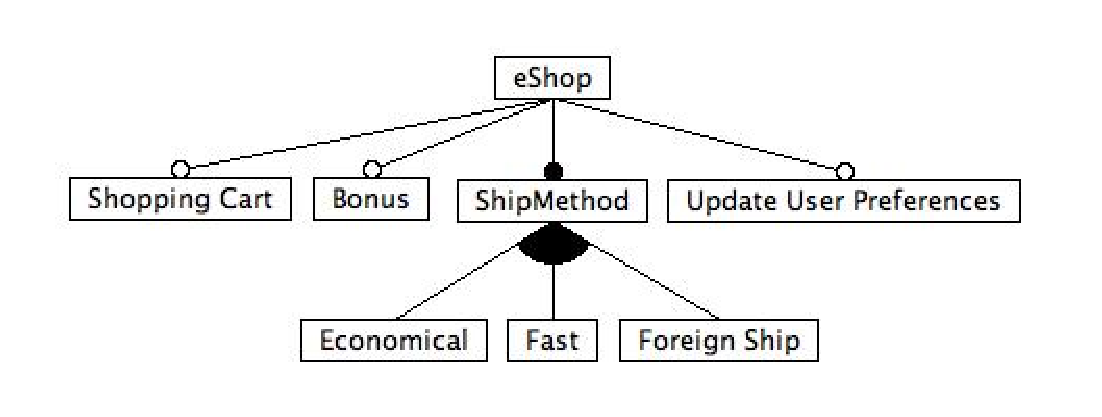
\includegraphics[scale=0.40]{../images/eShop-fm-re.eps}
   \caption{Subset of eShop feature model.}
  \label{fig:eshop-fm-re}
  \end{center}
\end{figure}

Notice that \emph{Proceed to Purchase} and \emph{Search for Products} scenarios
are mandatory (Table~\ref{tab:ck-running-example}), since they are related to a feature
expression that allways hold true (the root feature). Other scenarios will
be present only if the related expression is evaluated as \emph{true} for
the specific product being generated.

\begin{table}[tbh]
\begin{center}
 \caption{eShop configuration knowledge}
\label{tab:ck-running-example}
\begin{tabular}{ll}
   \hline\noalign{\smallskip}
  {\bf Expression} & {\bf Required Scenarios} \\
   \noalign{\smallskip}
   \hline
   \noalign{\smallskip}
    eShop & Proceed to Purchase \\
               & Search for Products \\
               & \ldots \\ 
    {\bf not} (Cart {\bf and} Bonus)\hspace{2pt} & Buy a Product \\ 
    Cart {\bf and} Bonus & Buy Products with Cart \\ 
    Update Preferences & Register User Preferences	 \\  
    \ldots & \ldots \\ 
  \hline
\end{tabular}
\end{center}
\end{table}

Listing~\ref{lst:configure} presents the product derivation function
(\emph{pdWeaver}), which corresponds to the reference implementation for
\emph{optional use cases and scenarios} technique. This function takes as input a
\emph{SPL use case model} (UCM), a \emph{feature model} (FM), a \emph{product
configuration} (PC), and a \emph{configuration knowledge} (CK).

\begin{lstlisting}[belowskip=20pt,frame=tb,caption={Product derivation weaver function},label=lst:configure]
pdWeaver :: UCM -> FM -> PC -> CK -> ScenarioList
pdWeaver ucm fm pc ck = 
 if not (validInstance fm pc) 
  then error InvalidProduct
  else retrieveScenarios ucm (configure pc ck)

configure :: PC -> CK -> ListOfScenarioId
configure pc (CK []) = []
configure pc (CK (x:xs)) =
 if (eval pc (expression x))
  then (artifacts x) ++ (configure pc (CK xs))
  else configure pc (CK xs)
\end{lstlisting} 

Initially, this function verifies if the product configuration is a well formed
instance of the feature model (Line 3 in Listing~\ref{lst:configure}) --- if it is not
the case,  an \emph{InvalidProduct} error is thrown. Then, the IDs of selected
scenarios are computed by the \emph{configure} function. This is done by
evaluating which feature expressions, defined in the list elements (x:xs) of
the configuration knowledge, are valid for the specific product instance
(\emph{eval} function). Finally, given the resulting list of scenario IDs, the function
\emph{retrieveScenarios} returns the product specific scenarios. 

It is important to notice that this variation technique presents two levels of
crosscutting. First, the feature model, the product configuration, and
the configuration knowledge crosscut each other with respect to the
list of valid scenario IDs. Then, the resulting list of scenario IDs crosscuts
with the use case model for selecting the product specific scenarios.   

The model of the \emph{optional use cases and scenarios} technique, in terms of
our modeling framework, is shown in Table~\ref{tab:pd-weaver}. The
\emph{pdWeaver} function is used to argue that the model is realizable and
appropriate. We achieve this by matching the model elements to corresponding parameters 
and auxiliary functions in the reference implementation. Therefore, the input languages UCM,
FM, CK, and PC are represented as different parameters of the \emph{pdWeaver}
function. An instance of the UCM corresponds to the specification of all SPL
scenarios. A FM instance is only responsible for declaring the SPL features and
the relationships between them. As a consequence, there is no coupling between
FMs and UCMs. Instead, relationships between features and artifacts are
documented in the configuration knowledge. Finally, the PC specifies which
features were selected for a specific product. 

The UCM has a greater importance over the other input languages ($UCM_{EFF}$),
since it declares the product specific scenarios (the output of this weaver
process generated by the \emph{pdWeaver} function). These scenarios ($UCM_{ID}$) are used
in the \emph{retrieveScenarios} function in order to identify which artifacts
will be assembled in the final product.

In order to identify which artifacts are required for a specific product, the
\emph{configure} function ($CK_{EFF}$) checks the feature expression ($CK_{ID}$)
against the product specific features ($PC_{ID}$). The effect of FM in this
weaver ($FM_{EFF}$) is to check if the PC is well formed. Such evaluation is
implemented by the \emph{validInstance} function and considers the PC feature
selection ($PC_{EFF}$). 

\begin{table}[htb]
\begin{center}
 \caption{Model of Product Derivation} \label{tab:pd-weaver}
\begin{tabular}{p{0.6in}p{2.4in}}
   \hline\noalign{\smallskip}
  {\bf Element} & {\bf Description} \\
   \noalign{\smallskip}
   \hline
   \noalign{\smallskip}
   $o$               & Product specific scenarios (list of scenarios) \\ 
   $o_{jp}$        & Scenario declarations \\ 
   $L$               & \{UCM, FM, CK, PC\} \\ 
   $UCM_{ID}$ & SPL scenarios \\ 
   $FM_{ID}$    & SPL features \\ 
   $CK_{ID}$    & Feature expressions and scenario IDs\\  
   $PC_{ID}$    & Product specific feature selection \\ 
   $UCM_{EFF}$ & Provides declaration of scenarios \\  
   $FM_{EFF}$    & Checks if a SPL instance is well formed \\ 
   $CK_{EFF}$    & Identifies selected artifacts  \\ 
   $PC_{EFF}$    &Triggers scenario selection \\
   $UCM_{MOD}$ & Scenario \\  
   $FM_{MOD}$   & Feature \\ 
   $CK_{MOD}$    & Each pair $(expression, artifact\ list)$  \\ 
   $PC_{MOD}$    & Feature \\
  \hline
  \end{tabular}
\end{center}
\end{table}



% -------------------------------------------------------------------------
\section{Evaluation}\label{sec:evaluation}


%-------------------------------------------------------------------------
\section{Related work}\label{sec:related}

\section{Concluding remarks}\label{sec:concludings}

%------------------------------------------------------------------------- 

\bibliographystyle{latex8}
\bibliography{../references/phd-references}

\end{document}

